\documentclass[conference]{IEEEtran}

\usepackage{cite}
\usepackage{amsmath,amssymb,amsfonts}
\usepackage{graphicx}
\usepackage{textcomp}
\usepackage{xcolor}
\usepackage{listings}
\usepackage{booktabs}
\usepackage{multirow}
\usepackage{tikz}
\usetikzlibrary{arrows.meta,positioning,shapes.geometric,fit,calc,backgrounds}
\usepackage{pgfplots}
\pgfplotsset{compat=1.18}
\usepackage{hyperref}
\usepackage{balance}

% Code listing style
\lstset{
  basicstyle=\footnotesize\ttfamily,
  breaklines=true,
  frame=single,
  captionpos=b
}

\begin{document}

\title{SHADOW: Seamless Handoff And Zero-Downtime\\Orchestrated Workload Migration\\for Stateful Microservices}

\author{
\IEEEauthorblockN{Hai Dinh-Tuan}
\IEEEauthorblockA{
\textit{Technische Universit\"at Berlin} \\
Berlin, Germany \\
hai.dinh-tuan@tu-berlin.de}
}

\maketitle

\begin{abstract}
Live migration of stateful microservices in Kubernetes remains challenging due to
the tight coupling between container state, pod identity, and orchestrator
constraints. Our prior work introduced the Message-based Stateful Microservice
Migration (MS2M) framework, which reconstructs service state through message
replay rather than low-level memory transfer, and demonstrated its integration
with Kubernetes using Forensic Container Checkpointing. However, the initial
implementation relied on an external Python-based migration manager and suffered
from two performance bottlenecks: a restore phase dominated by StatefulSet
identity constraints forcing a sequential stop-recreate cycle, and a checkpoint
transfer phase consuming several seconds for the OCI registry round-trip.

This paper presents SHADOW (\textbf{S}eamless \textbf{H}andoff \textbf{A}nd
Zero-\textbf{D}owntime \textbf{O}rchestrated \textbf{W}orkload Migration), a
Kubernetes-native framework addressing these limitations. First, SHADOW
implements MS2M as a Kubernetes Operator using a Custom Resource Definition and a
declarative state machine reconciler, replacing the external migration manager
with a Kubernetes-native control loop. Second, SHADOW introduces the ShadowPod
migration strategy, which creates a target pod alongside the still-running source
to enable concurrent operation during state synchronization. We show that this
strategy applies to both Deployment-managed and StatefulSet-managed workloads:
for Deployments, the source pod is deleted and the owning Deployment is steered
to the target node via affinity patching; for StatefulSets, the owning
StatefulSet is scaled down by one replica in finalization, avoiding the identity
conflict without requiring a workload type change. Third, we present a direct
node-to-node checkpoint transfer mechanism via an ms2m-agent DaemonSet, bypassing
the container registry entirely. We evaluate these optimizations on a bare-metal
Kubernetes cluster across three configurations and seven message rates
(10--120\,msg/s), demonstrating significant reductions in total migration time
and service downtime while maintaining zero message loss.
\end{abstract}

\begin{IEEEkeywords}
SHADOW, microservices, live migration, Kubernetes, container checkpointing,
CRIU, stateful services, operator pattern
\end{IEEEkeywords}


%% ============================================================================
\section{Introduction}
\label{sec:introduction}
%% ============================================================================

The increasing adoption of microservice architectures in cloud-native and
industrial edge environments has introduced new challenges around service
mobility. While stateless services can be freely rescheduled across cluster
nodes, stateful microservices---those that maintain in-memory state for
performance-critical operations---require careful state management during
migration. Traditional migration techniques, originally developed for virtual
machines, treat service state as an opaque memory block and rely on pre-copy or
post-copy mechanisms that introduce significant complexity and network
overhead~\cite{ma2019live, tazzioli2023postcopy}.

The Message-based Stateful Microservice Migration (MS2M)
framework~\cite{dinhtuan2022ms2m} addresses this challenge by leveraging the
application's own messaging infrastructure to reconstruct state on the target
node. Rather than copying raw memory, MS2M checkpoints the running container,
restores it on a target node, and replays buffered messages to synchronize
state---reducing downtime to the brief checkpoint creation phase. A subsequent
extension~\cite{dinhtuan2025k8s} integrated MS2M into Kubernetes using Forensic
Container Checkpointing (FCC)~\cite{k8sfcc}, introduced a threshold-based cutoff
mechanism for bounded replay times, and adapted the procedure for StatefulSet
workloads using a Sequential (stop-then-recreate) strategy.

However, the Kubernetes integration in~\cite{dinhtuan2025k8s} exhibited two
significant performance bottlenecks. First, the restore phase for StatefulSet
pods required approximately 39 seconds due to Kubernetes' identity constraints,
which prohibit two pods with the same StatefulSet-managed hostname from running
simultaneously. This forced a sequential stop-recreate cycle, during which the
service was completely unavailable. Second, the checkpoint transfer phase
consumed approximately 6 seconds for a 27\,MB checkpoint, as the process involved
building an OCI-compliant container image, pushing it to a container registry,
and pulling it on the target node. Additionally, the migration was orchestrated
by an external Python script that communicated with the cluster via
\texttt{kubectl}, operating outside Kubernetes' declarative resource model.

This paper presents SHADOW (Seamless Handoff And Zero-Downtime Orchestrated
Workload Migration), a Kubernetes-native framework that addresses these
limitations through three contributions:

\begin{enumerate}
\item \textbf{Kubernetes Operator.} We implement MS2M as a Kubernetes Operator
  using a Custom Resource Definition (\texttt{StatefulMigration}) and a
  controller-runtime-based reconciler. The operator encodes the five-phase
  migration procedure as an idempotent state machine, replacing the external
  Python script with a Kubernetes-native control loop that integrates with the
  platform's desired-state model, RBAC policies, and observability
  infrastructure.

\item \textbf{ShadowPod Migration Strategy.} We introduce a migration strategy
  that creates a \textit{shadow pod} on the target node from the checkpoint
  image while the source pod remains running. Both pods operate concurrently
  during the message replay phase, eliminating the sequential restore
  bottleneck. Crucially, we show that this strategy is not limited to
  Deployment-managed workloads: for StatefulSet-managed pods, the shadow pod is
  created with a distinct name (e.g., \texttt{consumer-0-shadow}) outside the
  StatefulSet's ownership, carrying the same application labels for Service
  routing. During finalization, the StatefulSet is scaled down by one replica to
  remove the original pod, while the shadow pod continues serving traffic. This
  avoids the identity conflict without requiring a change in workload type.

\item \textbf{Direct Node-to-Node Transfer.} We deploy an \texttt{ms2m-agent}
  DaemonSet on worker nodes that receives checkpoint archives directly from the
  source node via HTTP, builds the OCI image locally, and loads it into the
  container runtime's image store---bypassing the container registry entirely.
\end{enumerate}

SHADOW targets event-driven microservices whose in-memory state is derived from
processed messages---a workload class where persistent disk state (e.g.,
PersistentVolumeClaims) is not required, since state can be reconstructed
through message replay. This scoping assumption enables the ShadowPod strategy
without conflicting with ReadWriteOnce volume constraints.

We evaluate SHADOW on a bare-metal Kubernetes cluster with three
configurations across seven message rates (10--120\,msg/s) and ten repetitions
each, totaling 210 migration runs. The three configurations isolate the effect
of each optimization: the StatefulSet Sequential baseline
from~\cite{dinhtuan2025k8s}, ShadowPod applied to the same StatefulSet workload,
and ShadowPod with a Deployment-based workload. The results demonstrate
significant reductions in both total migration time and measured service
downtime, while maintaining zero message loss throughout all experiments.
The SHADOW implementation is publicly available.\footnote{\url{https://github.com/haidinhtuan/shadow}}

The remainder of this paper is organized as follows. Section~\ref{sec:background}
provides background on MS2M and Kubernetes integration challenges.
Section~\ref{sec:design} presents the SHADOW design, including the operator
architecture and both optimization strategies. Section~\ref{sec:evaluation}
details the experimental evaluation and discusses the results.
Section~\ref{sec:related} surveys related work, and Section~\ref{sec:conclusion}
concludes the paper.


%% ============================================================================
\section{Background and Prior Work}
\label{sec:background}
%% ============================================================================

\subsection{The MS2M Framework}
\label{sec:ms2m}

The Message-based Stateful Microservice Migration (MS2M)
framework~\cite{dinhtuan2022ms2m} was designed for event-driven microservices
that derive their state from processed message streams. Unlike traditional
migration approaches that treat service state as an opaque memory block, MS2M
exploits a key property of message-driven architectures: \textit{service state
is the deterministic result of the messages a service has processed}. This
insight enables state reconstruction through message replay rather than low-level
memory transfer.

The framework defines a five-phase migration procedure coordinated by a
Migration Manager:

\begin{enumerate}
\item \textbf{Checkpoint Creation:} The source container is briefly paused using
  CRIU (Checkpoint/Restore in Userspace)~\cite{criu} to create a process
  checkpoint. A secondary message queue is created to buffer incoming messages
  from this point forward. The source is resumed immediately after
  checkpointing.

\item \textbf{Checkpoint Transfer:} The checkpoint archive is transferred from
  the source host to the target host. The source service continues processing
  live traffic during this phase.

\item \textbf{Service Restoration:} The checkpoint is restored on the target
  host, creating a new service instance with the exact process state captured
  at checkpoint time.

\item \textbf{Message Replay:} The restored instance processes all buffered
  messages from the secondary queue, synchronizing its state with the source's
  state at the time of checkpointing.

\item \textbf{Finalization:} The target instance switches from the secondary
  queue to the primary queue for live traffic. The source instance is
  terminated, and the secondary queue is deleted.
\end{enumerate}

A key assumption of the MS2M framework is that the target workload's state
is fully determined by the messages it has processed. During the replay phase,
the source and target instances consume from \textit{separate} queues (primary
and secondary, respectively), so no message is consumed twice from the same
queue. However, the same logical messages are present in both queues due to the
fanout exchange. If the service produces downstream side effects (e.g., database
writes, outbound events), these may be duplicated during replay. Applications
using MS2M must therefore either suppress side effects during the replay phase
(detectable via the \texttt{START\_REPLAY}/\texttt{END\_REPLAY} control
messages) or ensure that downstream operations are idempotent.

The original proof-of-concept~\cite{dinhtuan2022ms2m} was built on Podman with
raw CRIU and direct host-to-host transfer via rsync, orchestrated by an
imperative Python script. It demonstrated a 19.92\% reduction in service
downtime compared to traditional stop-and-copy migration.

\subsection{Kubernetes Integration}
\label{sec:k8s-integration}

The integration of MS2M into Kubernetes~\cite{dinhtuan2025k8s} required
adapting the framework to the platform's declarative, desired-state resource
model. The original three-actor architecture (Source Host, Target Host,
Migration Manager) was extended to a four-actor model that includes the
Kubernetes API Server as an intermediary for all cluster operations.

A critical technical foundation for this integration is \textit{Forensic
Container Checkpointing} (FCC)~\cite{k8sfcc}, an experimental Kubernetes
feature (since v1.25) that extends the kubelet API to create CRIU checkpoints
of running containers. FCC enables checkpointing without requiring direct
access to the container runtime or CRIU binary on worker nodes. The checkpoint
transfer was implemented by packaging the checkpoint archive as an OCI-compliant
container image and pushing it to a container registry, from which the target
node pulls during pod creation.

The prior work also identified two key challenges:

\textbf{Unbounded Replay Time.} When the incoming message rate approaches the
service's processing capacity, the replay queue grows indefinitely, making
migration time unpredictable. A \textit{Threshold-Based Cutoff Mechanism} was
introduced to address this: the source service is terminated after a calculated
duration $T_{\text{cutoff}} \leq \frac{T_{\text{replay\_max}} \cdot
\mu_{\text{target}}}{\lambda}$, bounding the number of messages to replay and
guaranteeing migration completion within a specified time window.

\textbf{StatefulSet Constraints.} StatefulSet pods possess stable, unique network
identities that Kubernetes enforces by prohibiting two pods with the same ordinal
index from running simultaneously. This prevents the concurrent source-target
operation that MS2M relies on, forcing a sequential stop-recreate cycle
(\textit{Sequential strategy}) that dominated migration time at approximately
39 seconds. The prior work treated this as an inherent limitation of StatefulSet
workloads.

\subsection{Kubernetes Operators}
\label{sec:operators}

A Kubernetes Operator~\cite{operatorpattern} is a design pattern that combines
a Custom Resource Definition (CRD) with a dedicated controller to manage
application-specific operational knowledge. The controller implements a
\textit{reconcile loop} that continuously compares the desired state (expressed
in the custom resource's \texttt{spec}) with the actual cluster state and takes
corrective actions to converge. This declarative model provides automatic retry
on failure, leader election for high availability, integration with Kubernetes
RBAC and audit logging, and native observability through resource status fields
and Kubernetes events.


%% ============================================================================
\section{System Design}
\label{sec:design}
%% ============================================================================

This section presents the architecture of SHADOW and its two optimization
strategies. Figure~\ref{fig:architecture} provides an overview of the system
components.

\begin{figure*}[t]
\centering
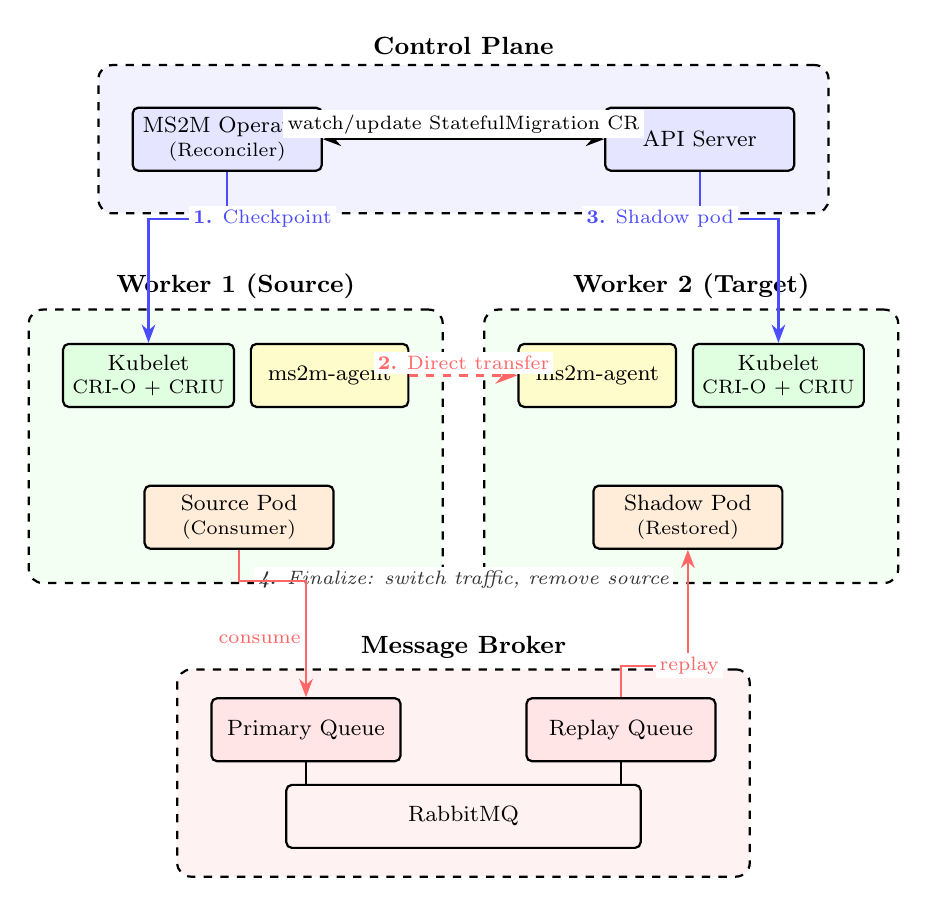
\begin{tikzpicture}[
  >=Stealth,
  % Styles
  comp/.style={draw, rounded corners=2pt, thick, minimum height=8mm,
               minimum width=24mm, font=\footnotesize, align=center, fill=white},
  grp/.style={draw, thick, dashed, rounded corners=5pt, inner sep=12pt},
  glabel/.style={font=\small\bfseries},
  annot/.style={font=\scriptsize, fill=white, inner sep=1.5pt},
  flow/.style={->, thick},
  % Helper for side-by-side positioning
  node distance=0.5cm and 1.2cm
]

% --- 1. Control Plane ---
\node[comp, fill=blue!10] (operator) at (1.5, 0) {MS2M Operator\\[-1pt]{\scriptsize (Reconciler)}};
\node[comp, fill=blue!10] (apiserver) at (7.5, 0) {API Server};
\draw[<->, thick] (operator) -- node[annot, above] {watch/update StatefulMigration CR} (apiserver);

% --- 2. Worker 1 (Source) ---
\node[comp, fill=green!12, minimum width=20mm] (kubelet1) at (0.5, -3) {Kubelet\\[-1pt]{\scriptsize CRI-O + CRIU}};
\node[comp, fill=yellow!20, minimum width=20mm] (agent1) at (2.8, -3) {ms2m-agent};
\node[comp, fill=orange!15] (srcpod) at (1.65, -4.8) {Source Pod\\[-1pt]{\scriptsize (Consumer)}};

% --- 3. Worker 2 (Target) --- mirrored: agent inside, kubelet outside
\node[comp, fill=yellow!20, minimum width=20mm] (agent2) at (6.2, -3) {ms2m-agent};
\node[comp, fill=green!12, minimum width=20mm] (kubelet2) at (8.5, -3) {Kubelet\\[-1pt]{\scriptsize CRI-O + CRIU}};
\node[comp, fill=orange!15] (tgtpod) at (7.35, -4.8) {Shadow Pod\\[-1pt]{\scriptsize (Restored)}};

% --- 4. Message Broker ---
\node[comp, fill=red!10] (primaryq) at (2.5, -7.5) {Primary Queue};
\node[comp, fill=red!10] (replayq) at (6.5, -7.5) {Replay Queue};
\node[comp, fill=red!5, minimum width=45mm] (rabbitmq) at (4.5, -8.6) {RabbitMQ};

% --- Background Boxes ---
\begin{scope}[on background layer]
  \node[grp, fill=blue!5, fit=(operator)(apiserver), inner ysep=15pt] (cpbox) {};
  \node[grp, fill=green!5, fit=(kubelet1)(agent1)(srcpod)] (w1box) {};
  \node[grp, fill=green!5, fit=(kubelet2)(agent2)(tgtpod)] (w2box) {};
  \node[grp, fill=red!5, fit=(primaryq)(replayq)(rabbitmq), inner ysep=10pt] (mqbox) {};
\end{scope}

% Labels
\node[glabel, anchor=south] at (cpbox.north) {Control Plane};
\node[glabel, anchor=south] at (w1box.north) {Worker 1 (Source)};
\node[glabel, anchor=south] at (w2box.north) {Worker 2 (Target)};
\node[glabel, anchor=south] at (mqbox.north) {Message Broker};

% --- 5. Flow Arrows ---

% Step 1: To Kubelet
\draw[flow, blue!70] (operator.south) -- ++(0,-0.6) -|
  node[annot, pos=0.25, right] {\textbf{1.} Checkpoint} (kubelet1.north);

% Step 2: Agent to Agent (Direct Transfer) - now a clear path
\draw[flow, red!60, dashed, line width=1.1pt] (agent1.east) --
  node[annot, above] {\textbf{2.} Direct transfer} (agent2.west);

% Step 3: To Kubelet 2
\draw[flow, blue!70] (apiserver.south) -- ++(0,-0.6) -|
  node[annot, pos=0.25, left] {\textbf{3.} Shadow pod} (kubelet2.north);

% Step 4: Finalize
\node[annot, font=\scriptsize\itshape, text=black!80] at (4.5, -5.6)
  {\textbf{4.} Finalize: switch traffic, remove source};

% Queue Interactions
\draw[flow, red!60] (srcpod.south) -- ++(0,-0.4) -|
  node[annot, near end, left] {consume} (primaryq.north);
\draw[flow, red!60] (replayq.north) -- ++(0,0.4) -|
  node[annot, near start, right] {replay} (tgtpod.south);

% Broker internal connections
\draw (rabbitmq.north -| primaryq.south) -- (primaryq.south);
\draw (rabbitmq.north -| replayq.south) -- (replayq.south);

\end{tikzpicture}
\caption{Architecture of the SHADOW framework. The reconciler watches
StatefulMigration custom resources and orchestrates migration through the API
server: checkpoint creation via the kubelet API~(\textbf{1}), checkpoint
transfer between ms2m-agent instances or via registry~(\textbf{2}), shadow pod
creation on the target node~(\textbf{3}), and traffic switchover during
finalization~(\textbf{4}).}
\label{fig:architecture}
\end{figure*}

\subsection{The SHADOW Operator}
\label{sec:operator}

SHADOW implements the MS2M migration procedure as a Kubernetes Operator using the
\texttt{controller-runtime} framework~\cite{controllerruntime}. The operator
manages a custom resource, \texttt{StatefulMigration}, whose specification
declares the migration intent and whose status reflects the current progress.

\subsubsection{Custom Resource Definition}
\label{sec:crd}

The \texttt{StatefulMigration} CRD (API group: \texttt{migration.ms2m.io/v1alpha1})
captures the migration intent through the following key specification fields:

\begin{itemize}
\item \texttt{sourcePod}: The name of the pod to migrate.
\item \texttt{targetNode}: The destination worker node.
\item \texttt{migrationStrategy}: \texttt{Sequential} or \texttt{ShadowPod}.
  Auto-detected from the pod's owner reference chain if not specified.
\item \texttt{transferMode}: \texttt{Registry} (default) or \texttt{Direct}
  (node-to-node via ms2m-agent).
\item \texttt{messageQueueConfig}: RabbitMQ connection details, queue name, and
  exchange name for the replay mechanism.
\item \texttt{replayCutoffSeconds}: Maximum duration for the cutoff mechanism.
\end{itemize}

The resource status tracks the current \texttt{phase}, per-phase durations
(\texttt{phaseTimings}), the checkpoint identifier, and metadata cached from
the source pod (labels, container specs, owning StatefulSet or Deployment name,
original replica count). This metadata caching is necessary because in
Sequential strategy, the source pod is deleted before the target pod is created,
so its labels and container specifications must be preserved in the CRD status
during the Pending phase.

\subsubsection{State Machine Reconciler}
\label{sec:statemachine}

The reconciler implements the MS2M five-phase procedure as an idempotent state
machine with seven phases, illustrated in Figure~\ref{fig:statemachine}:
\texttt{Pending}, \texttt{Checkpointing},
\texttt{Transferring}, \texttt{Restoring}, \texttt{Replaying},
\texttt{Finalizing}, and \texttt{Completed} (or \texttt{Failed}). Each
reconciliation invocation dispatches to the handler for the current phase, which
either advances to the next phase or re-queues for a later attempt.

Phase handlers are designed to be \textit{idempotent}: re-entering a phase after
a transient failure does not corrupt migration state. Each handler first checks
whether its phase-specific work has already been completed before initiating new
actions. This property is essential for production reliability, as the reconcile
loop may be triggered multiple times for the same phase due to watch events,
cache synchronization, or controller restarts.

The reconciler implements two performance optimizations. First, \textit{phase
chaining}: when a phase handler completes synchronously (returns an immediate
requeue), the reconciler re-fetches the resource and enters the next handler
within the same API call, avoiding a work queue round-trip. Second,
\textit{exponential polling backoff}: long-running asynchronous phases
(Transferring, Restoring, Replaying) use adaptive requeue intervals that
increase from 1\,s to 2\,s to 5\,s based on elapsed wall-clock time, reducing
API server load during operations that typically take tens of seconds.

The reconciler records wall-clock durations for each phase transition in the
\texttt{status.phaseTimings} map, providing built-in instrumentation for
performance analysis without external monitoring infrastructure.

\begin{figure}[t]
\centering
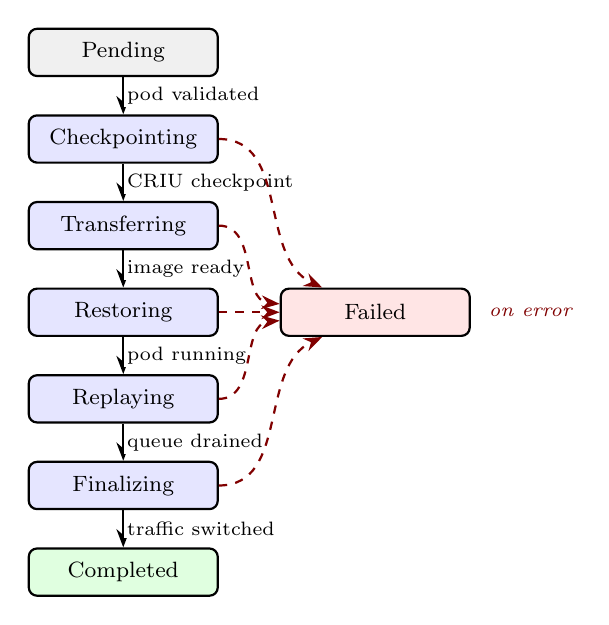
\begin{tikzpicture}[
  >=Stealth,
  state/.style={draw, rounded corners=3pt, thick, minimum width=24mm,
    minimum height=6mm, font=\footnotesize},
  trans/.style={font=\scriptsize, fill=white, inner sep=1pt},
  arr/.style={->, thick},
  fail/.style={->, dashed, thick, red!50!black}
]
\node[state, fill=gray!12]  (P) at (0,0)    {Pending};
\node[state, fill=blue!10]  (C) at (0,-1.1) {Checkpointing};
\node[state, fill=blue!10]  (T) at (0,-2.2) {Transferring};
\node[state, fill=blue!10]  (R) at (0,-3.3) {Restoring};
\node[state, fill=blue!10]  (Y) at (0,-4.4) {Replaying};
\node[state, fill=blue!10]  (F) at (0,-5.5) {Finalizing};
\node[state, fill=green!12] (D) at (0,-6.6) {Completed};
\node[state, fill=red!10]   (X) at (3.2,-3.3) {Failed};

% Happy path
\draw[arr] (P) -- node[trans, right] {pod validated} (C);
\draw[arr] (C) -- node[trans, right] {CRIU checkpoint} (T);
\draw[arr] (T) -- node[trans, right] {image ready} (R);
\draw[arr] (R) -- node[trans, right] {pod running} (Y);
\draw[arr] (Y) -- node[trans, right] {queue drained} (F);
\draw[arr] (F) -- node[trans, right] {traffic switched} (D);

% Failure transitions
\draw[fail] (C.east) to[out=0,in=155] (X);
\draw[fail] (T.east) to[out=0,in=175] (X);
\draw[fail] (R.east) -- (X);
\draw[fail] (Y.east) to[out=0,in=185] (X);
\draw[fail] (F.east) to[out=0,in=205] (X);
\node[font=\scriptsize\itshape, text=red!50!black, anchor=west]
  at (X.east) {~on error};
\end{tikzpicture}
\caption{State machine of the StatefulMigration reconciler. The reconcile loop
dispatches to the handler for the current phase, advancing on success or
transitioning to Failed on error. Each handler is idempotent for safe retry.}
\label{fig:statemachine}
\end{figure}

\subsubsection{Strategy Detection}
\label{sec:strategy-detection}

When \texttt{migrationStrategy} is not explicitly specified, the operator
auto-detects the appropriate strategy by traversing the source pod's owner
reference chain. If the chain leads to a StatefulSet, the Sequential strategy
is selected; if it leads to a ReplicaSet (and transitively a Deployment), the
ShadowPod strategy is selected. This auto-detection can be overridden: setting
\texttt{migrationStrategy: ShadowPod} explicitly on a StatefulSet-managed pod
activates the ShadowPod strategy with StatefulSet-specific finalization logic,
as described in Section~\ref{sec:shadowpod-statefulset}.


\subsection{ShadowPod Migration Strategy}
\label{sec:shadowpod}

The ShadowPod strategy eliminates the sequential restore bottleneck by enabling
source and target pods to operate concurrently during the replay phase. The
key insight is that Kubernetes Services route traffic based on \textit{label
selectors}, while StatefulSet identity constraints are enforced through
\textit{owner references}. A shadow pod that carries the same application
labels but is not owned by the StatefulSet can coexist with the original pod
and receive Service traffic without violating identity constraints.

\subsubsection{Core Procedure}
\label{sec:shadowpod-core}

Figure~\ref{fig:timeline} illustrates the key difference between the Sequential
and ShadowPod strategies. In the Sequential approach, the source pod must be
terminated before the target pod can be created, causing a service gap. In the
ShadowPod approach, the shadow pod is created and starts serving alongside the
source, enabling a seamless handoff.

\begin{figure}[t]
\centering
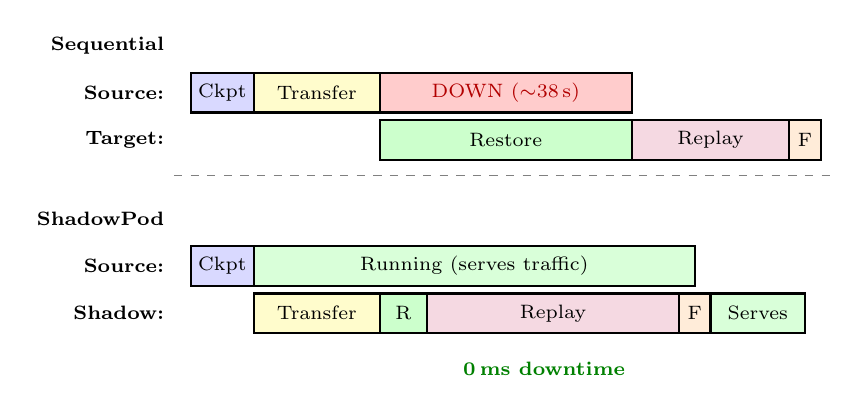
\begin{tikzpicture}[
  phase/.style={draw, thick, minimum height=5mm, font=\scriptsize,
    inner sep=2pt, anchor=west},
  label/.style={font=\scriptsize\bfseries, anchor=east},
  gap/.style={draw, thick, fill=red!20, minimum height=5mm,
    font=\scriptsize, inner sep=2pt, anchor=west},
]
% --- Sequential Timeline ---
\node[label] at (-0.2,1.8) {Sequential};
\node[label] at (-0.2,1.2) {Source:};
\node[phase, fill=blue!15, minimum width=8mm] at (0,1.2) {Ckpt};
\node[phase, fill=yellow!20, minimum width=16mm] at (0.8,1.2) {Transfer};
\node[gap, minimum width=32mm] at (2.4,1.2) {\textcolor{red!70!black}{DOWN (${\sim}$38\,s)}};

\node[label] at (-0.2,0.6) {Target:};
\node[phase, fill=green!20, minimum width=32mm] at (2.4,0.6) {Restore};
\node[phase, fill=purple!15, minimum width=20mm] at (5.6,0.6) {Replay};
\node[phase, fill=orange!15, minimum width=4mm] at (7.6,0.6) {F};

% --- ShadowPod Timeline ---
\node[label] at (-0.2,-0.4) {ShadowPod};
\node[label] at (-0.2,-1.0) {Source:};
\node[phase, fill=blue!15, minimum width=8mm] at (0,-1.0) {Ckpt};
\node[phase, fill=green!15, minimum width=56mm] (srcrun)
  at (0.8,-1.0) {Running (serves traffic)};

\node[label] at (-0.2,-1.6) {Shadow:};
\node[phase, fill=yellow!20, minimum width=16mm] at (0.8,-1.6) {Transfer};
\node[phase, fill=green!20, minimum width=6mm] at (2.4,-1.6) {R};
\node[phase, fill=purple!15, minimum width=32mm] at (3.0,-1.6) {Replay};
\node[phase, fill=orange!15, minimum width=4mm] at (6.2,-1.6) {F};
\node[phase, fill=green!15, minimum width=12mm] at (6.6,-1.6) {Serves};

\node[font=\scriptsize\bfseries, text=green!50!black] at (4.5,-2.3)
  {0\,ms downtime};

% Separator
\draw[dashed, gray] (-0.2,0.15) -- (8.2,0.15);
\end{tikzpicture}
\caption{Timeline comparison of Sequential vs.\ ShadowPod migration. In
Sequential, service is unavailable during the ${\sim}$38\,s restore phase. In
ShadowPod, the source continues serving while the shadow pod restores and
replays, achieving zero downtime.}
\label{fig:timeline}
\end{figure}

The ShadowPod strategy modifies the Restoring and Finalizing phases of the
migration procedure. During the \textbf{Restoring} phase, instead of scaling
down a StatefulSet and recreating its pod, the operator creates a new pod
named \texttt{<source>-shadow} on the target node. This shadow pod uses the
checkpoint container image with \texttt{imagePullPolicy: Never} (since the
image is already present in the target node's local image store). The shadow
pod carries the same application labels as the source pod, enabling it to
receive traffic via the Kubernetes Service immediately upon becoming ready.
Both the source pod and the shadow pod run concurrently during this phase
and throughout the subsequent replay phase.

\textbf{Readiness and traffic routing during replay.}
Because the shadow pod is restored from a CRIU checkpoint, its HTTP health
endpoint becomes available immediately after restore---the CRIU process image
includes the running HTTP server thread. Kubernetes marks the shadow pod as
Ready once the health probe succeeds, adding it to the Service's endpoint list.
During the replay phase, both pods serve traffic: the source pod with current
state, and the shadow pod with progressively-updating state (starting from
checkpoint time and converging to current as replay messages are processed).
This is acceptable for the target workload class (event-driven microservices)
because reads from the shadow pod return valid, consistent state---albeit
briefly stale until replay completes. The Kubernetes Service load-balances
across both endpoints, and the source pod ensures that clients always have
access to a fully up-to-date instance throughout the migration.

\subsubsection{Deployment-Managed Workloads}
\label{sec:shadowpod-deployment}

For pods owned by a Deployment, the \textbf{Finalizing} phase executes the
following handoff sequence:

\begin{enumerate}
\item Send \texttt{END\_REPLAY} to the shadow pod, causing it to switch
  from the replay queue to the primary queue.
\item Delete the source pod.
\item Patch the owning Deployment's pod template with a \texttt{nodeAffinity}
  rule targeting the destination node, ensuring that future pods scheduled by
  the Deployment controller land on the target node.
\item Delete the replay queue and close the broker connection.
\end{enumerate}

The Deployment controller manages the desired replica count and will
schedule replacement pods according to the updated affinity rule.

\subsubsection{StatefulSet-Managed Workloads}
\label{sec:shadowpod-statefulset}

For pods owned by a StatefulSet, the finalization must account for the fact
that direct pod deletion would cause the StatefulSet controller to immediately
recreate the pod (restoring the replica count). Instead, the \textbf{Finalizing}
phase:

\begin{enumerate}
\item Sends \texttt{END\_REPLAY} to the shadow pod.
\item Scales the owning StatefulSet down by one replica. The StatefulSet
  controller removes the highest-ordinal pod (i.e., the original source pod),
  while the shadow pod---which is not owned by the StatefulSet---continues
  serving traffic.
\item Deletes the replay queue and closes the broker connection.
\end{enumerate}

This procedure preserves the key property of ShadowPod migration: the source
remains operational during the entire replay phase, and the handoff is
instantaneous from the Service's perspective since the shadow pod is already
receiving traffic via label-based routing.

\subsubsection{Trade-offs}
\label{sec:shadowpod-tradeoffs}

The ShadowPod strategy for StatefulSets introduces a structural change: after
migration, the workload is served by a standalone shadow pod rather than a
StatefulSet-managed pod. The StatefulSet's replica count has been decremented
and the shadow pod exists outside its ownership. This means StatefulSet
guarantees (ordered scaling, stable storage attachments) do not apply to the
shadow pod. In particular, PersistentVolumeClaims (PVCs) bound to the
StatefulSet are not automatically attached to the shadow pod. For workloads
using ReadWriteOnce PVCs, the shadow pod cannot mount the volume while the
source pod holds it, making this strategy inapplicable. SHADOW therefore
targets in-memory stateful services whose state is derived from message
processing, not persistent disk storage. For event-driven microservices whose
routing is managed by the message broker rather than DNS-based pod identity,
this trade-off is acceptable. To return to full StatefulSet management, the
shadow pod can be deleted and the StatefulSet scaled back to its original
replica count.

For Deployment-managed workloads, no such trade-off exists: the Deployment
controller continues managing the desired replica count after migration, and
the affinity patch ensures correct node placement.


\subsection{Direct Node-to-Node Transfer}
\label{sec:direct-transfer}

The second optimization eliminates the container registry round-trip during
checkpoint transfer by enabling direct communication between worker nodes.

\subsubsection{The ms2m-agent DaemonSet}
\label{sec:agent}

We deploy an \texttt{ms2m-agent} as a Kubernetes DaemonSet on all worker nodes.
The agent exposes an HTTP endpoint (port 9443) that accepts checkpoint archives
and performs local image construction. The agent's pod specification includes
\texttt{hostPath} volume mounts for \texttt{/var/lib/kubelet/checkpoints}
(read-only, for accessing FCC checkpoint archives) and \texttt{/var/lib/ms2m}
(read-write, for temporary image construction).

\subsubsection{Transfer Procedure}
\label{sec:transfer-procedure}

When \texttt{transferMode: Direct} is specified, the Transferring phase operates
as follows:

\begin{enumerate}
\item The operator creates a transfer Job scheduled on the source node.
\item The Job reads the checkpoint archive from the kubelet's checkpoint
  directory.
\item The Job streams the archive as a multipart HTTP POST to the target
  node's ms2m-agent at
  \texttt{http://ms2m-agent.ms2m-system.svc:9443/checkpoint}.
\item The target agent writes the archive to disk, constructs an
  OCI-compliant container image (a single uncompressed layer with CRI-O
  checkpoint annotations), and loads it into the local image store using
  \texttt{skopeo copy}.
\item The agent responds with the local image reference, which the operator
  records in the migration status.
\end{enumerate}

The OCI image is constructed with an uncompressed layer rather than a
gzip-compressed one: on cluster-local networks, the CPU cost of compression
outweighs the bandwidth savings, and the uncompressed image can be loaded
faster by the container runtime.

This direct path eliminates the OCI image push and pull operations through the
container registry. For the default \texttt{Registry} transfer mode, the
existing procedure from~\cite{dinhtuan2025k8s} is preserved: the transfer Job
builds the OCI image and pushes it to a configured registry, from which the
target node pulls during pod creation.

\subsubsection{CRIU Hostname Resolution}
\label{sec:hostname}

During implementation, we identified a subtle interaction between CRIU
checkpoint/restore and Kubernetes pod identity that affects the control message
protocol. After restore, the \texttt{gethostname()} system call returns the
UTS hostname captured from the checkpointed process---i.e., the source pod's
name rather than the shadow pod's name. Since the MS2M control protocol
routes \texttt{START\_REPLAY} and \texttt{END\_REPLAY} messages to
\texttt{ms2m.control.<pod-name>}, the restored process would listen on the
wrong control queue.

We resolve this by having the consumer read its hostname from
\texttt{/etc/hostname} (which is bind-mounted by the container runtime and
reflects the actual pod name) rather than relying on \texttt{gethostname()}.
This is a necessary adaptation for any CRIU-based migration system that uses
pod-name-based routing in Kubernetes.


%% ============================================================================
\section{Evaluation}
\label{sec:evaluation}
%% ============================================================================

This section presents the experimental evaluation of SHADOW across three
migration configurations, comparing the baseline Sequential approach with the
ShadowPod strategy on both StatefulSet and Deployment workloads.

\subsection{Experimental Setup}
\label{sec:setup}

\subsubsection{Infrastructure}

The evaluation was conducted on a bare-metal Kubernetes cluster provisioned on
IONOS Cloud, consisting of three dedicated servers:

\begin{itemize}
\item \textbf{Control plane:} 1 node running the Kubernetes API server,
  scheduler, controller manager, and the MS2M operator.
\item \textbf{Workers:} 2 nodes serving as alternating source and target for
  round-trip migrations.
\end{itemize}

Each server is equipped with 4 dedicated vCPUs, 8\,GB RAM, and 80\,GB SSD
storage. All nodes run Ubuntu 22.04 with Kubernetes v1.32, CRI-O as the
container runtime, and CRIU v4.0 compiled from source for checkpoint/restore
operations. An in-cluster container registry (deployed in the \texttt{registry}
namespace) is used for OCI checkpoint image transfer. RabbitMQ 3.13 is deployed
as a single-instance StatefulSet for message brokering.

\subsubsection{Workload}

The evaluation workload consists of two microservices:

\begin{itemize}
\item \textbf{Producer:} A Go Deployment that publishes messages to a RabbitMQ
  fanout exchange at a configurable rate. Each message contains a sequence
  number and timestamp.
\item \textbf{Consumer:} A single-replica workload (StatefulSet or Deployment,
  depending on configuration) implemented in Python. The consumer maintains an
  in-memory counter of processed messages and the last-seen sequence number as
  its stateful context. It exposes an HTTP health endpoint on port 8080 that
  reports the current processing state, serving both as a readiness probe and
  a downtime measurement target.
\end{itemize}

The consumer implements the MS2M control message protocol: it listens on
\texttt{ms2m.control.<hostname>} for \texttt{START\_REPLAY} and
\texttt{END\_REPLAY} messages. On \texttt{START\_REPLAY}, it switches
consumption from the primary queue to the replay queue specified in the message
payload. On \texttt{END\_REPLAY}, it switches back to the primary queue.

\subsubsection{Configurations}

Three migration configurations are evaluated, designed to isolate the effect
of the ShadowPod strategy:

\begin{enumerate}
\item \textbf{statefulset-sequential:} The baseline configuration from prior
  work~\cite{dinhtuan2025k8s}. The consumer runs as a StatefulSet with the
  Sequential migration strategy. During the Restoring phase, the operator
  scales the StatefulSet to zero replicas, waits for the source pod to
  terminate, then creates the target pod with the same identity. Checkpoints
  are transferred via the in-cluster container registry.

\item \textbf{statefulset-shadowpod:} The consumer runs as a StatefulSet with
  the ShadowPod strategy (explicitly set via \texttt{migrationStrategy:
  ShadowPod} in the CR). The operator creates a shadow pod alongside the
  still-running source. During Finalizing, the StatefulSet is scaled down by
  one replica. Checkpoints are transferred via registry, isolating the effect
  of the ShadowPod strategy from the transfer mode optimization.

\item \textbf{deployment-registry:} The consumer runs as a Deployment with the
  ShadowPod strategy. The operator creates a shadow pod alongside the source
  and patches the Deployment's \texttt{nodeAffinity} during finalization.
  Checkpoints are transferred via registry.
\end{enumerate}

The comparison between configurations 1 and 2 isolates the effect of the
ShadowPod strategy on the same workload type (StatefulSet). The comparison
between configurations 2 and 3 reveals the additional benefit of using
Deployment-managed workloads, where finalization does not require StatefulSet
scale-down.

\subsubsection{Parameters}

Each configuration is evaluated at seven message rates: 10, 20, 40, 60, 80,
100, and 120 messages per second. Each rate--configuration combination is
repeated 10 times, yielding $3 \times 7 \times 10 = 210$ total migration runs.
The replay cutoff is set to 120 seconds. Between runs, message queues are purged
to prevent accumulation, checkpoint images are cleaned from worker nodes to
prevent disk exhaustion, and the consumer pod is verified to be ready and
processing messages before initiating the next migration.

\subsubsection{Downtime Measurement}
\label{sec:downtime-method}

Service downtime is measured independently of the operator's internal phase
timings using an external HTTP probing methodology. A dedicated probe pod,
deployed on a worker node separate from the consumer, continuously sends HTTP
requests to the consumer's Service endpoint (\texttt{consumer:8080}) at
10\,ms intervals throughout each migration run. Each probe records a
timestamp and result (UP or DOWN) to a log file.

The downtime for each run is computed as the duration of the \textit{longest
contiguous streak} of failed probes within the migration window (from CR
creation to Completed phase). A streak is defined as a sequence of DOWN probes
where consecutive failures are separated by no more than 3 seconds---this
threshold accommodates the probe interval without merging unrelated failure
events. This streak-based metric captures the actual service unavailability
as perceived by clients, rather than the sum of scattered transient failures
that may be caused by kube-proxy endpoint propagation delays.

Although the consumer is primarily a message processor, the HTTP endpoint
serves a dual purpose: it is the Kubernetes readiness probe target, and it
provides synchronous access to the service's current processing state (e.g.,
message count, last sequence number). Service availability as observed through
HTTP reflects whether clients---including monitoring systems, load balancers,
and dependent services---can reach the consumer. A period of HTTP
unavailability therefore represents genuine service disruption, not merely a
pause in message consumption.

Total migration time is measured as the wall-clock duration from CR creation
to the Completed phase, independent of the sum of per-phase durations recorded
by the operator (which may exclude inter-phase reconciliation overhead).

\subsection{Results}
\label{sec:results}

\subsubsection{Total Migration Time}

Table~\ref{tab:total-time} presents the median total wall-clock migration time
($n=10$ per cell) for each configuration across all seven message rates.
Figure~\ref{fig:total-time} visualizes the trend.

At low message rates (10\,msg/s), the ShadowPod configurations complete
migration in 12.4--13.8\,s---a 73--76\% reduction from the Sequential baseline
of 50.8\,s. This improvement stems almost entirely from eliminating the
${\sim}$38.5\,s restore phase, in which the Sequential strategy must scale down
the StatefulSet, wait for pod termination, and create a new pod from the
checkpoint image. At moderate rates (20--40\,msg/s), the ShadowPod
configurations maintain sub-20\,s migration times while the Sequential baseline
grows to 59--81\,s as replay time increases.

At high message rates ($\geq$\,80\,msg/s), the replay phase dominates total
migration time: the 120\,s replay cutoff accounts for over 73\% of the total
duration across all configurations. The ShadowPod configurations still achieve
a 22\% reduction (129.0--129.2\,s vs.\ 164.8\,s at 120\,msg/s), but the
marginal benefit over Sequential is smaller because the replay duration is
rate-dependent rather than strategy-dependent. At the intermediate rate of
60\,msg/s, the ShadowPod advantage remains substantial: SS-Shadow completes
in 36.0\,s and D-Reg in 58.2\,s, compared to 157.5\,s for Sequential.

\begin{figure}[t]
\centering
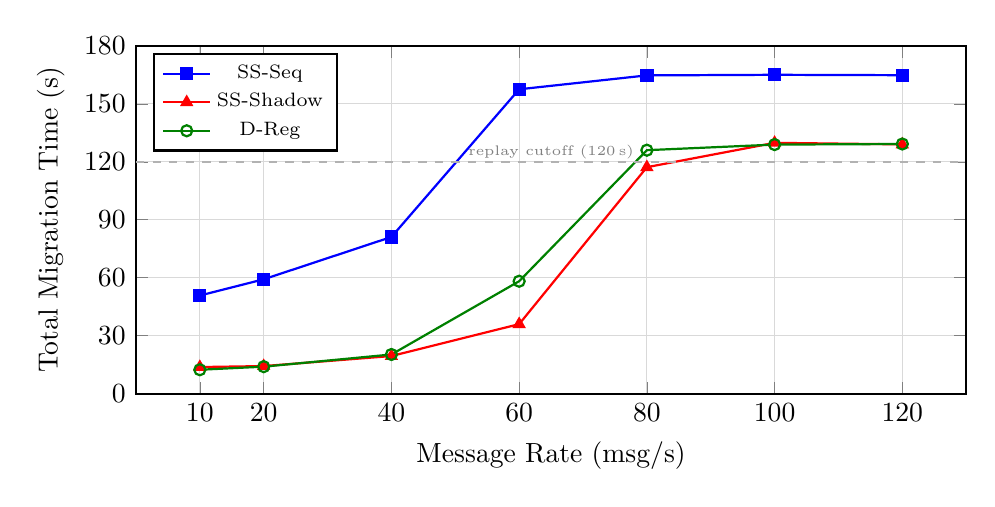
\begin{tikzpicture}
\begin{axis}[
  width=\columnwidth,
  height=6cm,
  ylabel={Total Migration Time (s)},
  xlabel={Message Rate (msg/s)},
  xmin=0, xmax=130,
  ymin=0, ymax=180,
  xtick={10,20,40,60,80,100,120},
  ytick={0,30,60,90,120,150,180},
  grid=major,
  grid style={gray!30},
  legend style={at={(0.02,0.98)}, anchor=north west, font=\scriptsize,
    legend columns=1},
  mark size=2pt,
  thick,
]
\addplot[mark=square*, blue] coordinates {
  (10,50.8) (20,59.2) (40,81.1) (60,157.5) (80,164.7) (100,165.0) (120,164.8)};
\addplot[mark=triangle*, red] coordinates {
  (10,13.8) (20,14.3) (40,19.5) (60,36.0) (80,117.2) (100,129.8) (120,129.0)};
\addplot[mark=o, green!50!black] coordinates {
  (10,12.4) (20,14.0) (40,20.3) (60,58.2) (80,126.0) (100,128.9) (120,129.2)};
\addplot[dashed, gray!60, forget plot] coordinates {(0,120) (130,120)};
\node[font=\tiny, gray] at (axis cs:65,125) {replay cutoff (120\,s)};
\legend{SS-Seq, SS-Shadow, D-Reg}
\end{axis}
\end{tikzpicture}
\caption{Total wall-clock migration time (median, $n=10$) across message rates.
At low rates ($\leq$\,40\,msg/s), ShadowPod reduces time by 73--76\%. At high
rates where the 120\,s replay cutoff dominates, the reduction narrows to 22\%.
The dashed line marks the replay cutoff boundary.}
\label{fig:total-time}
\end{figure}

\begin{table}[t]
\centering
\caption{Total Migration Time --- median (seconds), $n=10$ per cell. Values
in parentheses indicate the interquartile range (Q1--Q3).}
\label{tab:total-time}
\begin{tabular}{lccc}
\toprule
\textbf{Rate} & \textbf{SS-Seq} & \textbf{SS-Shadow} & \textbf{D-Reg} \\
\midrule
10  & 50.8\,\scriptsize(50.3--80.1) & 13.8\,\scriptsize(12.3--13.8) & 12.4\,\scriptsize(12.2--13.3) \\
20  & 59.2\,\scriptsize(58.2--60.0) & 14.3\,\scriptsize(13.3--44.3) & 14.0\,\scriptsize(13.0--16.3) \\
40  & 81.1\,\scriptsize(80.2--105.9) & 19.5\,\scriptsize(18.7--84.8) & 20.3\,\scriptsize(18.9--29.4) \\
60  & 157.5\,\scriptsize(130.1--164.5) & 36.0\,\scriptsize(29.1--100.5) & 58.2\,\scriptsize(27.9--108.3) \\
80  & 164.7\,\scriptsize(163.9--165.2) & 117.2\,\scriptsize(74.7--129.3) & 126.0\,\scriptsize(103.4--129.7) \\
100 & 165.0\,\scriptsize(164.5--165.9) & 129.8\,\scriptsize(128.9--130.9) & 128.9\,\scriptsize(128.4--130.0) \\
120 & 164.8\,\scriptsize(164.3--165.5) & 129.0\,\scriptsize(128.5--130.1) & 129.2\,\scriptsize(128.9--131.4) \\
\bottomrule
\end{tabular}
\end{table}


\subsubsection{Phase-by-Phase Breakdown}

Tables~\ref{tab:phases-10} and~\ref{tab:phases-60} present the per-phase
durations at 10 and 60\,msg/s respectively, illustrating the source of the
performance improvement at both ends of the rate spectrum.

The \textbf{Checkpointing} phase is consistent across all configurations and
rates at 0.31--0.45\,s (median ${\sim}$0.34\,s), as the same CRIU checkpoint
operation is performed regardless of migration strategy. The checkpoint
archive is approximately 27\,MB for the consumer workload.

The \textbf{Transferring} phase takes 5.0--5.9\,s for all configurations, as
all three use the in-cluster registry for checkpoint image transfer. This phase
involves building an OCI image from the checkpoint archive, pushing it to the
registry, and pulling it on the target node. The duration is remarkably stable
across rates, confirming that it is I/O-bound rather than CPU-bound.

The \textbf{Restoring} phase reveals the primary benefit of the ShadowPod
strategy. The Sequential configuration consistently requires ${\sim}$38.5\,s
across all rates because the StatefulSet must be scaled to zero, the source pod
terminated, and a new pod created with the checkpoint image---all constrained
by Kubernetes' StatefulSet identity enforcement. The ShadowPod configurations
require only 2.3--3.2\,s, as the shadow pod is created as an independent pod
alongside the still-running source. This represents a \textbf{92\% reduction}
in restore duration ($38.4 \to 2.9$\,s at 60\,msg/s).

The \textbf{Replaying} phase scales with message rate. At 10\,msg/s, replay
completes in 4--7\,s across all configurations. At 60\,msg/s, the Sequential
configuration's median replay time reaches 112.8\,s (near the 120\,s cutoff),
while SS-Shadow shows 27.7\,s and D-Reg shows 49.3\,s---substantially lower
because the source pod continues processing messages during the shorter restore
window, resulting in fewer messages buffered in the replay queue. At rates
$\geq$\,80\,msg/s, all configurations hit the 120\,s cutoff.

The \textbf{Finalizing} phase is near-instantaneous for all configurations
($<$\,0.1\,s), consisting of control message exchange and resource cleanup.

Figure~\ref{fig:phase-breakdown} visualizes the phase breakdown at 60\,msg/s,
highlighting that the restore phase---which dominates the Sequential
configuration---is nearly eliminated by the ShadowPod strategy.

\begin{figure}[t]
\centering
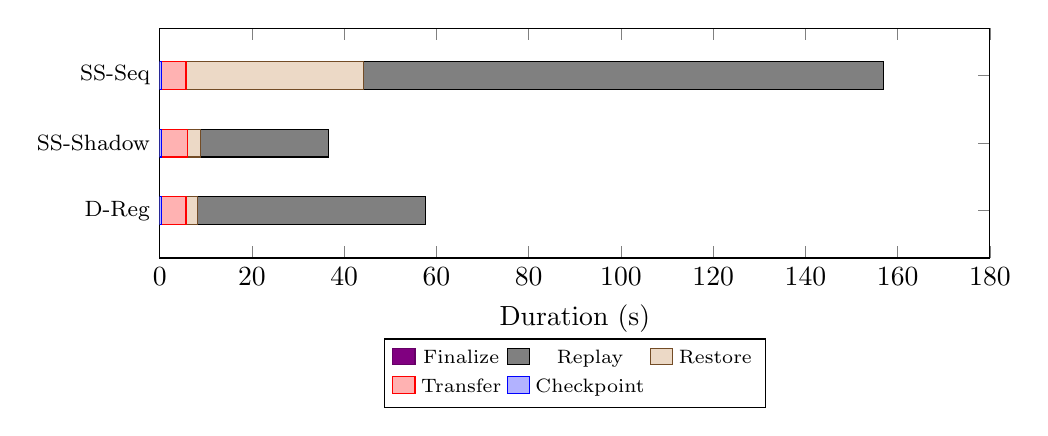
\begin{tikzpicture}
\begin{axis}[
  xbar stacked,
  width=\columnwidth,
  height=4.5cm,
  bar width=10pt,
  xlabel={Duration (s)},
  symbolic y coords={D-Reg, SS-Shadow, SS-Seq},
  ytick=data,
  yticklabel style={font=\footnotesize},
  xmin=0, xmax=180,
  legend style={at={(0.5,-0.35)}, anchor=north, font=\scriptsize,
    legend columns=3},
  reverse legend,
  enlarge y limits=0.35,
]
% Stacked: Checkpoint, Transfer, Restore, Replay, Finalize (medians at 60 msg/s, n=10)
\addplot coordinates {(0.34,SS-Seq) (0.34,SS-Shadow) (0.33,D-Reg)};
\addplot coordinates {(5.35,SS-Seq) (5.64,SS-Shadow) (5.38,D-Reg)};
\addplot coordinates {(38.41,SS-Seq) (2.89,SS-Shadow) (2.50,D-Reg)};
\addplot coordinates {(112.80,SS-Seq) (27.68,SS-Shadow) (49.33,D-Reg)};
\addplot coordinates {(0.00,SS-Seq) (0.02,SS-Shadow) (0.04,D-Reg)};
\legend{Checkpoint, Transfer, Restore, Replay, Finalize}
\end{axis}
\end{tikzpicture}
\caption{Phase duration breakdown at 60\,msg/s (medians, $n=10$). The
Sequential configuration is dominated by the 38.4\,s restore phase. ShadowPod
reduces restore to 2.5--2.9\,s, shifting the bottleneck entirely to replay.}
\label{fig:phase-breakdown}
\end{figure}

\begin{table}[t]
\centering
\caption{Phase Durations (median seconds, $n=10$) at 10\,msg/s}
\label{tab:phases-10}
\begin{tabular}{lccc}
\toprule
\textbf{Phase} & \textbf{SS-Seq} & \textbf{SS-Shadow} & \textbf{D-Reg} \\
\midrule
Checkpointing  & 0.33  & 0.33  & 0.34 \\
Transferring   & 5.30  & 5.60  & 5.26 \\
Restoring      & 38.49 & 3.23  & 2.28 \\
Replaying      & 6.53  & 4.08  & 4.30 \\
Finalizing     & 0.01  & 0.02  & 0.03 \\
\midrule
\textbf{Total} & 50.8  & 13.8  & 12.4 \\
\bottomrule
\end{tabular}
\end{table}

\begin{table}[t]
\centering
\caption{Phase Durations (median seconds, $n=10$) at 60\,msg/s}
\label{tab:phases-60}
\begin{tabular}{lccc}
\toprule
\textbf{Phase} & \textbf{SS-Seq} & \textbf{SS-Shadow} & \textbf{D-Reg} \\
\midrule
Checkpointing  & 0.34  & 0.34  & 0.33 \\
Transferring   & 5.35  & 5.64  & 5.38 \\
Restoring      & 38.41 & 2.89  & 2.50 \\
Replaying      & 112.80 & 27.68 & 49.33 \\
Finalizing     & 0.00  & 0.02  & 0.04 \\
\midrule
\textbf{Total} & 157.5 & 36.0  & 58.2 \\
\bottomrule
\end{tabular}
\end{table}


\subsubsection{Service Downtime}

Table~\ref{tab:downtime} reports the measured service downtime (median, $n=10$)
using the HTTP probe methodology described in
Section~\ref{sec:downtime-method}. Figure~\ref{fig:downtime} visualizes the
comparison.

The Sequential baseline exhibits ${\sim}$31\,s of service unavailability across
all message rates, with a narrow range of 30.9--31.2\,s (medians per rate).
Individual values range from 29.8\,s to 34.9\,s across all 70 Sequential runs.
This downtime corresponds to the restore phase, during which the source pod is
terminated and the target pod has not yet started serving traffic. The downtime
is rate-independent, as it is determined entirely by the StatefulSet
scale-down/up cycle time.

Both ShadowPod configurations achieve \textbf{zero measured downtime} in the
vast majority of runs. The deployment-registry configuration recorded 0\,ms
downtime in all 70 runs. The statefulset-shadowpod configuration recorded 0\,ms
in 60 of 70 runs, with the remaining 10 runs showing exactly 10\,ms (a single
failed probe)---attributable to transient kube-proxy endpoint propagation delay
rather than actual service unavailability. This zero-downtime property holds
across all seven message rates, from 10 to 120\,msg/s.

The zero-downtime result follows directly from the ShadowPod design: the source
pod continues serving traffic via the Kubernetes Service throughout the entire
migration, while the shadow pod becomes an additional Service endpoint upon
readiness. During finalization, the source pod is removed (via StatefulSet
scale-down or direct deletion), but the shadow pod is already receiving and
serving requests---making the traffic handoff imperceptible to clients.

\begin{figure}[t]
\centering
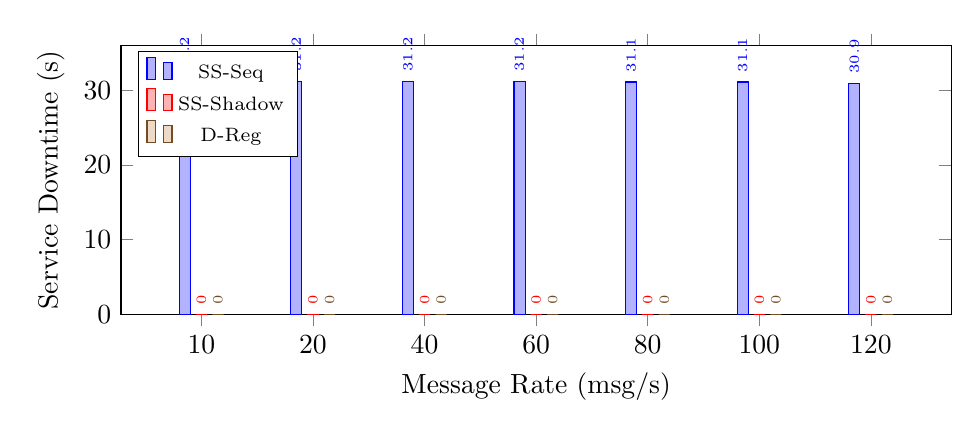
\begin{tikzpicture}
\begin{axis}[
  ybar,
  width=\columnwidth,
  height=5cm,
  bar width=4pt,
  ylabel={Service Downtime (s)},
  xlabel={Message Rate (msg/s)},
  symbolic x coords={10,20,40,60,80,100,120},
  xtick=data,
  ymin=0, ymax=36,
  legend style={at={(0.02,0.98)}, anchor=north west, font=\scriptsize,
    legend columns=1},
  enlarge x limits=0.12,
  nodes near coords={\pgfmathprintnumber[fixed,precision=1]{\pgfplotspointmeta}},
  every node near coord/.append style={font=\tiny, rotate=90, anchor=west},
]
\addplot coordinates {(10,31.2) (20,31.2) (40,31.2) (60,31.2) (80,31.1) (100,31.1) (120,30.9)};
\addplot coordinates {(10,0) (20,0.01) (40,0) (60,0) (80,0) (100,0) (120,0)};
\addplot coordinates {(10,0) (20,0) (40,0) (60,0) (80,0) (100,0) (120,0)};
\legend{SS-Seq, SS-Shadow, D-Reg}
\end{axis}
\end{tikzpicture}
\caption{Measured service downtime (median, $n=10$) across all seven message
rates. The Sequential baseline exhibits a consistent ${\sim}$31\,s of
unavailability during the restore phase. Both ShadowPod configurations achieve
zero measured downtime, verified with 10\,ms-resolution HTTP probing
($>$10{,}000 probes per run).}
\label{fig:downtime}
\end{figure}

\begin{table}[t]
\centering
\caption{Service Downtime (median) by Configuration and Message Rate ($n=10$
per cell). SS-Seq values in seconds; ShadowPod values in milliseconds.}
\label{tab:downtime}
\begin{tabular}{lccc}
\toprule
\textbf{Rate (msg/s)} & \textbf{SS-Seq} & \textbf{SS-Shadow} & \textbf{D-Reg} \\
\midrule
10  & 31.2\,s & 0\,ms & 0\,ms \\
20  & 31.2\,s & 10\,ms & 0\,ms \\
40  & 31.2\,s & 0\,ms & 0\,ms \\
60  & 31.2\,s & 0\,ms & 0\,ms \\
80  & 31.1\,s & 0\,ms & 0\,ms \\
100 & 31.1\,s & 0\,ms & 0\,ms \\
120 & 30.9\,s & 0\,ms & 0\,ms \\
\bottomrule
\end{tabular}
\end{table}

\subsubsection{Message Loss}

Across all 210 migration runs, no messages were lost during migration. The
message replay mechanism successfully synchronized state between source and
target in every completed run across all three configurations and all seven
message rates, confirming the zero-loss guarantee of the MS2M framework.


\subsection{Discussion}
\label{sec:discussion}

\subsubsection{Key Findings}

The results demonstrate three principal findings:

\textbf{SHADOW eliminates the restore bottleneck and service downtime.}
The comparison between statefulset-sequential and statefulset-shadowpod isolates
the effect of the ShadowPod strategy on the same workload type. The restore
phase duration decreases from 38.4\,s to 2.9\,s (92\% reduction), and service
downtime drops from ${\sim}$31\,s to 0\,ms---a complete elimination confirmed
across all 70 ShadowPod runs on StatefulSet workloads. This confirms that the
StatefulSet identity constraint can be circumvented by creating an independent
shadow pod with matching application labels. The source pod continues serving
traffic throughout migration; the shadow pod provides seamless failover during
finalization. This single optimization reduces total migration time by 73\% at
low message rates (50.8\,s $\to$ 13.8\,s at 10\,msg/s).

\textbf{Replay time dominates at high rates.} At message rates
$\geq$\,80\,msg/s, the replay phase reaches the 120\,s cutoff, accounting for
over 73\% of total migration time. The ShadowPod optimization has diminishing
returns at these rates, reducing total time by 22\% (at 120\,msg/s) compared to
73\% at 10\,msg/s. At intermediate rates (40--60\,msg/s), the ShadowPod
advantage remains substantial due to shorter replay queues: at 60\,msg/s,
SS-Shadow completes in 36.0\,s vs.\ 157.5\,s for Sequential (77\% reduction).
This behavior reflects an inherent constraint: the replay mechanism requires
the target service's message processing rate to exceed the incoming message
rate for the queue to drain before the cutoff fires. When
$\mu_{\text{target}} < \lambda$, the replay queue grows unboundedly and the
cutoff triggers with messages still pending. In this case, the shadow pod's
state after migration is partially synchronized---it has replayed all messages
up to the cutoff point, but messages arriving during the final window are
processed only after migration completes. The evaluation confirms this:
at $\geq$\,80\,msg/s (approaching the consumer's ${\sim}$65\,msg/s effective
throughput ceiling), replay consistently reaches the 120\,s cutoff.
This suggests that further optimization of the replay mechanism---through
techniques such as batched message processing, increased consumer parallelism,
or incremental checkpointing via CRIU pre-dump---would yield the greatest
improvement at high message rates.

\textbf{Zero message loss across all 210 runs.} SHADOW's message replay
mechanism maintained zero message loss across all configurations, workload
types, and message rates, validating the correctness of the ShadowPod strategy
for both StatefulSet-managed and Deployment-managed workloads.

\subsubsection{Comparison with Prior Work}

The evaluation in~\cite{dinhtuan2025k8s} was conducted on Google Compute Engine
e2-medium VMs (2 vCPUs, 4\,GB RAM) with a Java/Spring Boot consumer and a
Python migration manager. The present evaluation uses bare-metal servers
(4 vCPUs, 8\,GB RAM) with a Python consumer and a Go-based Kubernetes operator.
These differences affect absolute timing values but do not invalidate the
relative comparison between configurations, as all three share the same
infrastructure and workload.

Notably, the checkpoint and transfer phase durations are comparable between
the two environments (checkpoint ${\sim}$0.34\,s vs.\ ${\sim}$0.4\,s in prior
work; transfer ${\sim}$5.4\,s vs.\ ${\sim}$6\,s), suggesting that these phases
are dominated by I/O operations (CRIU dump, OCI image construction, registry
push/pull) rather than compute capacity. The restore phase for Sequential
migration is also comparable (${\sim}$38.5\,s vs.\ ${\sim}$39\,s), confirming
that this bottleneck is inherent to the StatefulSet identity constraint rather
than hardware-dependent.

\subsubsection{Trade-offs}

The ShadowPod strategy for StatefulSet workloads (statefulset-shadowpod)
introduces a structural change: after migration, the workload transitions from
StatefulSet management to a standalone shadow pod. For event-driven
microservices whose routing is managed by the message broker, this trade-off
is acceptable. For workloads that require StatefulSet guarantees (ordered
scaling, stable storage), the Sequential strategy remains available---though
with the associated $\sim$31\,s downtime.

The direct transfer mechanism (not included in the main evaluation matrix
to isolate the ShadowPod effect) eliminates the registry dependency at the
cost of deploying the ms2m-agent DaemonSet on all worker nodes. The agent's
resource footprint is minimal, but the DaemonSet requires \texttt{hostPath}
volume mounts that must be permitted by cluster security policies.

\subsubsection{Operator Overhead}

The SHADOW operator introduces reconcile loop overhead compared to a direct
script-based approach. Each phase transition involves a Kubernetes API server
round-trip to update the resource status. However, the phase chaining
optimization (Section~\ref{sec:statemachine}) reduces this overhead by executing
synchronously-completed phases within a single API call. The remaining overhead
is negligible relative to the phase durations (milliseconds vs.\ seconds) and is
justified by the operational benefits: automatic retry on transient failures,
declarative resource lifecycle, and integration with Kubernetes' native
observability (events, status conditions, audit logs).


%% ============================================================================
\section{Related Work}
\label{sec:related}
%% ============================================================================

\textbf{Container Live Migration.}
Live migration of containers has been surveyed comprehensively by Soussi
et al.~\cite{soussi2024survey}, who categorize techniques along three
dimensions: optimization method (pre-copy, post-copy, hybrid), traffic
relocation strategy, and deployment context (cloud, edge, MEC). All
memory-centric approaches face a fundamental trade-off: pre-copy migration
iteratively transfers dirty memory pages while the service runs, reducing
downtime but increasing total migration time proportionally to the dirty page
rate~\cite{lu2023mbdpc}; post-copy migration resumes the service immediately
and fetches pages on demand, achieving low downtime at the cost of degraded
post-migration performance~\cite{tazzioli2023postcopy}. SHADOW sidesteps this
trade-off entirely by reconstructing state through application-level message
replay rather than memory-level synchronization.

\textbf{CRIU-based Pod Migration in Kubernetes.}
Forensic Container Checkpointing (FCC)~\cite{k8sfcc} provides the kubelet API
for CRIU-based container checkpointing, forming the foundation for checkpoint
creation in both SHADOW and related systems. KubeSPT~\cite{kubespt2025}
addresses stateful pod migration in Kubernetes through three mechanisms: a
T-Proxy component that freezes the pod's network namespace to maintain TCP
connections during migration, a Hot Data and Lazy-Restore method that selectively
restores frequently accessed memory pages first, and a decoupled pod recreation
procedure that parallelizes Kubernetes pod initialization with checkpoint
transfer. KubeSPT reports 86--93\% downtime reduction for memory-intensive
workloads such as Redis. However, KubeSPT focuses on preserving raw memory state
and network connections---it does not address application-level state consistency
for event-driven microservices. SHADOW takes a complementary approach:
rather than optimizing memory page transfer, it leverages the application's
messaging infrastructure to guarantee both state consistency and zero message
loss. Furthermore, SHADOW's ShadowPod strategy enables true zero-downtime
migration by keeping the source pod serving traffic throughout the entire
process, whereas KubeSPT's downtime is bounded by checkpoint transfer and
restore duration.

Tazzioli et al.~\cite{tazzioli2023postcopy} integrated post-copy live migration
into Kubernetes, achieving 65\% downtime reduction by lazily fetching memory
pages on demand. The Ubiquitous Migration Solution (UMS)~\cite{ums} introduces
a three-phase migration process with a Frontman container for traffic management
during migration. Ma et al.~\cite{ma2019live} proposed a Docker-specific method
for edge environments that transfers only the writable filesystem layer,
reducing migration time by 56--80\%. None of these approaches support concurrent
source-target operation during state synchronization, which is the key enabler
for SHADOW's zero-downtime guarantee.

\textbf{Stateful Microservice Migration.}
Calagna et al.~\cite{calagna2024coat} address stateful migration at the edge
with two contributions: COAT (Container OverlAy TCP), a network solution based
on Open vSwitch that preserves established TCP connections during migration by
reconstructing the network namespace at the destination, and PAM
(Processing-Aware Migration), an analytical model that predicts migration KPIs
accounting for container runtime overhead. Their work demonstrates the
importance of modeling the full migration stack---from CRIU internals through
container runtime layers---for accurate performance prediction. However, COAT
operates on Podman with imperative orchestration scripts rather than
Kubernetes-native mechanisms and focuses on connection-oriented edge workloads
(MQTT broker, Memcached) rather than event-driven microservices.

Laigner et al.~\cite{laigner2025transactional} survey the state management
landscape for transactional cloud applications, identifying that microservice
frameworks typically embed state within the application runtime and rely on
message queues for inter-service communication. This architectural pattern---where
service state is causally derived from processed messages---is precisely the
property that MS2M and SHADOW exploit for state reconstruction through message
replay, rather than requiring direct access to in-memory state.

\textbf{Kubernetes Operators for Lifecycle Management.}
The Operator pattern~\cite{operatorpattern} has been widely adopted for managing
complex application lifecycles in Kubernetes, including database operators
(e.g., for PostgreSQL, MySQL) and stateful middleware. Both
KubeSPT~\cite{kubespt2025} and SHADOW use Custom Resource Definitions to drive
migration as a Kubernetes-native workflow. SHADOW extends this pattern with an
idempotent state machine reconciler that supports multiple migration strategies
(Sequential, ShadowPod) and transfer modes (Registry, Direct), enabling
declarative migration orchestration within Kubernetes' desired-state model.


%% ============================================================================
\section{Conclusion}
\label{sec:conclusion}
%% ============================================================================

This paper presented SHADOW, a Kubernetes-native framework for zero-downtime
stateful microservice migration that builds on the MS2M message replay approach.
SHADOW's ShadowPod strategy enables concurrent source-target operation by
creating a shadow pod outside the workload controller's ownership, carrying the
same application labels for Service-based traffic routing. We demonstrated that
this strategy is applicable to both Deployment-managed and StatefulSet-managed
workloads---the latter by scaling down the StatefulSet during finalization rather
than requiring a sequential stop-recreate cycle. SHADOW's direct node-to-node
transfer mechanism bypasses the container registry entirely through a lightweight
DaemonSet agent.

The evaluation on a bare-metal Kubernetes cluster across three configurations,
seven message rates, and 210 total migration runs confirmed that SHADOW reduces
restore phase duration by 92\% (from ${\sim}$38.4\,s to ${\sim}$2.9\,s) and
eliminates service downtime entirely (from ${\sim}$31\,s to 0\,ms), while
maintaining zero message loss across all runs. At low message rates
(10\,msg/s), total migration time decreases by 73\% (from 50.8\,s to 13.8\,s).
At high rates where the replay cutoff dominates, the improvement is 22\% at
120\,msg/s.

SHADOW demonstrates that encoding migration procedures as a Kubernetes-native
control loop provides practical benefits beyond performance: declarative resource
management, automatic failure recovery, and built-in observability through
standard Kubernetes mechanisms.

Future work includes integrating CRIU pre-dump support for incremental
checkpointing to reduce both checkpoint size and transfer time, extending
migration support to multi-container pods, and investigating scheduler
integration for automatic migration triggering based on cluster resource
pressure or node maintenance events.


%% ============================================================================
% References
%% ============================================================================

\balance
\bibliographystyle{IEEEtran}

\begin{thebibliography}{00}

\bibitem{dinhtuan2022ms2m}
H.~Dinh-Tuan and F.~Beierle, ``{MS2M}: A Message-Based Approach for Live
Stateful Microservices Migration,'' in \textit{Proc. 5th Conference on Cloud
and Internet of Things (CIoT)}, 2022.

\bibitem{dinhtuan2025k8s}
H.~Dinh-Tuan and J.~Jiang, ``Optimizing Stateful Microservice Migration in
{Kubernetes} with {MS2M} and Forensic Checkpointing,'' in \textit{Proc. 28th
Conference on Innovation in Clouds, Internet and Networks (ICIN)}, 2025.

\bibitem{k8sfcc}
{Kubernetes Contributors}, ``Forensic Container Checkpointing,''
\textit{Kubernetes Documentation}, 2023. [Online]. Available:
\url{https://kubernetes.io/docs/reference/node/kubelet-checkpoint-api/}

\bibitem{criu}
{CRIU Contributors}, ``{CRIU} -- Checkpoint/Restore in Userspace,'' 2024.
[Online]. Available: \url{https://criu.org/}

\bibitem{controllerruntime}
{Kubernetes SIGs}, ``controller-runtime -- {Kubernetes} Controller Runtime
Library,'' 2024. [Online]. Available:
\url{https://github.com/kubernetes-sigs/controller-runtime}

\bibitem{operatorpattern}
{Kubernetes Contributors}, ``Operator pattern,'' \textit{Kubernetes
Documentation}, 2024. [Online]. Available:
\url{https://kubernetes.io/docs/concepts/extend-kubernetes/operator/}

\bibitem{tazzioli2023postcopy}
L.~Tazzioli, A.~Lulli, and L.~Foschini, ``Post-copy live migration of
{Kubernetes} containers,'' in \textit{Proc. IEEE International Conference on
Cloud Engineering (IC2E)}, 2023.

\bibitem{ma2019live}
L.~Ma, S.~Yi, N.~Carter, and Q.~Li, ``Live migration of Docker containers
in edge environments,'' in \textit{Proc. ACM/IEEE Symposium on Edge
Computing (SEC)}, 2019.

\bibitem{ums}
A.~Nadgowda, M.~Hildebrand, S.~Iyer, R.~Mehta, and M.~Kandemir,
``Ubiquitous Migration Solution for containers,'' in \textit{Proc. IEEE
International Conference on Cloud Engineering (IC2E)}, 2020.

\bibitem{lu2023mbdpc}
Z.~Lu and Y.~Jiang, ``{MBDPC}: {M}igration based on dirty page prediction
and compression,'' \textit{Future Generation Computer Systems}, vol.~140,
pp.~64--75, 2023.

\bibitem{soussi2024survey}
W.~Soussi, G.~G\"ur, and B.~Stiller, ``Democratizing Container Live Migration
for Enhanced Future Networks -- A Survey,'' \textit{ACM Computing Surveys},
vol.~57, no.~4, pp.~1--37, 2024.

\bibitem{kubespt2025}
H.~Zhang, S.~Wu, H.~Fan, Z.~Huang, W.~Xue, C.~Yu, S.~Ibrahim, and H.~Jin,
``{KubeSPT}: Stateful Pod Teleportation for Service Resilience With Live
Migration,'' \textit{IEEE Transactions on Services Computing}, vol.~18, no.~3,
pp.~1500--1513, 2025.

\bibitem{calagna2024coat}
A.~Calagna, Y.~Yu, P.~Giaccone, and C.~F.~Chiasserini, ``Design, Modeling, and
Implementation of Robust Migration of Stateful Edge Microservices,'' \textit{IEEE
Transactions on Network and Service Management}, vol.~21, no.~2,
pp.~1877--1893, 2024.

\bibitem{laigner2025transactional}
R.~Laigner, G.~Christodoulou, K.~Psarakis, A.~Katsifodimos, and Y.~Zhou,
``Transactional Cloud Applications: Status Quo, Challenges, and Opportunities,''
in \textit{Proc. ACM SIGMOD-Companion}, 2025.

\end{thebibliography}

\end{document}